% -*- mode: latex; TeX-master: t; -*-

% \documentclass[notes=hide]{beamer}
% \documentclass[notes=only]{beamer}
\documentclass[
14pt,
aspectratio=169,
usenames,
dvipsnames,
% handout,
x11names]{beamer}
%\let\Tiny=\tiny

% Font selection
\overfullrule=5pt

\usepackage{etex}
\usepackage{pgfpages}

\usepackage{tabularx}
\usepackage{multicol}
% \usepackage[subfolder]{gnuplottex}

%% beamerscape dependencies
\usepackage[absolute,overlay]{textpos}
\setlength{\TPHorizModule}{\paperwidth}
\setlength{\TPVertModule}{\paperheight}
\textblockorigin{0mm}{0mm}

\definecolor{greenvm}{HTML}{AFD18E}
\definecolor{g}{HTML}{0E3B12}
\definecolor{v}{HTML}{003366}

\newcommand{\src}[1]{\scriptsize Figure Source: \textit{#1}}

%%%%%%%%%%%%%%%%%%%%%%%%%%%%%%%%%%%%%%%%%%%%%%%%%%%%%%%%%%%%%%%%%%%%%%%%%%%%%%%%
% Beamer template
\usetheme[
	bullet=square,             % Default option: circle
%	nobigpagenumber,         % No big circled page number on lower right
	noheadline,		 % No headline
%       nofootline,		 % No footline
	% grey,                    % For a neutral grey background color
%	watermark=BG_both,	 % png file for the watermark
]{Ithaca}
% \usetheme{metropolis}
% \usetheme{Boadilla}
%\usetheme{Berlin}
% \usetheme{Warsaw}
% % \usetheme{Dresden}
% %\usecolortheme{seagull}
% \usecolortheme{beaver}
% %\usecolortheme{seahorse}
%\usefonttheme{serif}
% \usefonttheme{structurebold}

%%%%%%%%%%%%%%%%%%%%%%%%%%%%%%%%%%%%%%%%%%%%%%%%%%%%%%%%%%%%%%%%%%%%%%%%%%%%%%%%
% Template
%%%%%%%%%%%%%%%%%%%%%%%%%%%%%%%%%%%%%%%%%%%%%%%%%%%%%%%%%%%%%%%%%%%%%%%%%%%%%%%%

\definecolor{mypurple}{HTML}{494949}
\definecolor{myyellow}{HTML}{FFCC33}
\definecolor{mygrey}{HTML}{999999}

\setbeamercolor{alerted text}{fg=myyellow}
\setbeamercolor{headline}{bg=footline.bg}
\setbeamercolor{block body alerted}{bg=normal text.bg!90!black}
\setbeamercolor{block body}{bg=normal text.bg!90!black}
\setbeamercolor{block body example}{bg=normal text.bg!90!black}
\setbeamercolor{block title alerted}{fg=myyellow}
\setbeamercolor{block title}{bg=blue}
\setbeamercolor{block title example}{use={normal text,example text},fg=example text.fg!75!normal text.fg,bg=normal text.bg!75!black}
\setbeamercolor{frametitle}{fg=white}
\setbeamercolor{item projected}{fg=white}
\setbeamercolor{normal text}{bg=mypurple,fg=white}
\setbeamercolor{section in sidebar}{fg=brown}
\setbeamercolor{section in sidebar shaded}{fg=grey}
\setbeamercolor{separation line}{}
\setbeamercolor{sidebar}{bg=red}
\setbeamercolor{sidebar}{parent=palette primary}
\setbeamercolor{structure}{bg=black, fg=white}
\setbeamercolor{subsection in sidebar}{fg=brown}
\setbeamercolor{subsection in sidebar shaded}{fg=grey}

% \setbeamercolor{palette primary}{fg=mypurple!80!black}
% \setbeamercolor{palette secondary}{fg=mypurple!80!black}
% \setbeamercolor{palette quaternary}{fg=mypurple!50!black}
% \setbeamercolor{page number in foot}{fg=white}

% lets add page numbers
% \expandafter\def\expandafter\insertshorttitle\expandafter{%
%   \insertshorttitle\hfill\insertframenumber\,/\,\inserttotalframenumber}

% \setbeamercovered{transparent}
\beamertemplatetransparentcoveredhigh

% *****************************************
% >>>> 15.3.2    Using Beamer's Templates
% *****************************************
% As a user of the beamer class you typically do not 'use' or 'invoke'
% templates yourself, directly. For example, the frame title template
% is automatically invoked by beamer somewhere deep inside the frame
% typesetting process. The same is true of most other
% templates. However, if, for whatever reason, you wish to invoke a
% template yourself, you can use the following command.
% \usebeamertemplate***{ element name }
% -------------------------------
%%% 7.2.1 The Headline and Footline
% \setbeamertemplate{headline} % Beamer-Template/-Color/-Font
% \setbeamertemplate{headline}
% {%
%   \begin{beamercolorbox}{section in head/foot}
%     \vskip2pt\insertnavigation{\paperwidth}\vskip2pt
%   \end{beamercolorbox}%
% }
% \setbeamertemplate{headline}[default] % The default is just an empty headline.
% \setbeamertemplate{headline}[infolines theme]
% \setbeamertemplate{headline}[miniframes theme]
% \setbeamertemplate{headline}[sidebar theme]
% \setbeamertemplate{headline}[smoothtree theme]
% \setbeamertemplate{headline}[smoothbars theme]
% \setbeamertemplate{headline}[tree]
% \setbeamertemplate{headline}[split theme]
% \setbeamertemplate{headline}[text line]{ text } % The headline is typeset with 'text'
% Logo in every slide except title
% \addtobeamertemplate{headline}{}
% {%
% \vspace{1ex}
% \hspace{1ex}
% \includegraphics[height=1cm]{myrmigki_color}
% }
% -------------------------------
% \setbeamertemplate{footline} % Beamer-Template/-Color/-Font
% \setbeamertemplate{footline}[default]
% \setbeamertemplate{footline}[infolines theme]
% \setbeamertemplate{footline}[miniframes theme]
% \setbeamertemplate{footline}[page number]
% \setbeamertemplate{footline}[frame number]
% \setbeamertemplate{footline}[split]
% \setbeamertemplate{footline}[text line]{ text }
% % Footline in every slideexcept title
\setbeamertemplate{footline}{
  \leavevmode%
  \begin{beamercolorbox}[left,wd=.4\paperwidth,ht=2.5ex,dp=1.125ex,leftskip=.3cm, rightskip=.3cm plus1fil]{footline}%
    \insertshorttitle%
  \end{beamercolorbox}
  %
  \begin{beamercolorbox}[center,wd=.2\paperwidth,ht=2.5ex,dp=1.125ex,leftskip=.3cm,rightskip=.3cm plus1fil]{footline}%
    \centering
    \insertframenumber~of~\inserttotalframenumber%
  \end{beamercolorbox}%
  %
  \begin{beamercolorbox}[right,wd=.4\paperwidth,ht=2.5ex,dp=1.125ex,leftskip=.3cm,rightskip=.3cm plus1fil]{footline}%
    \hskip2ex plus1fill%
    
\includegraphics[height=1.5ex]{cc}~%
    
\includegraphics[height=1.5ex]{by}~~%
    % 
\includegraphics[height=1.5ex]{sa}~~%
    \insertshortauthor~%
  \end{beamercolorbox}%
}%
% -------------------------------
%%% 7.2.2 The Sidebars
% -------------------------------
%%% 7.2.3 Navigation Bars (funktioniert nur mit miniframe Themes)
% \setbeamertemplate{mini frames}[default] % shows small circles as mini frames.
% \setbeamertemplate{mini frames}[box] % shows small rectangles as mini frames.
% \setbeamertemplate{mini frames}[tick] % shows small vertical bars as mini frames.
% -------------------------------
%%% 7.2.4 The Navigation Symbols
%%% Beamer-Template/-Color/-Font navigation symbols
% \setbeamertemplate{navigation symbols}{} % suppresses all navigation symbols:
% \setbeamertemplate{navigation symbols}[horizontal] % Organizes the navigation symbols horizontally.
% \setbeamertemplate{navigation symbols}[vertical] % Organizes the navigation symbols vertically.
% \setbeamertemplate{navigation symbols}[only frame symbol] % Shows only the navigational symbol for navigating frames.
% -------------------------------
%%% 7.2.5 The Logo
% \setbeamertemplate{logo} % Beamer-Template/-Color/-Font
% -------------------------------
%%% 7.2.6 The Frame Title
% \setbeamertemplate{frametitle} % Beamer-Template/-Color/-Font
% \setbeamertemplate{frametitle}[default][center] % left, center, right
% \setbeamertemplate{frametitle}[shadow theme]
% \setbeamertemplate{frametitle}[sidebar theme]
% \setbeamertemplate{frametitle}[smoothbars theme]
% \setbeamertemplate{frametitle}[smoothtree theme]
% \setbeamertemplate{frametitle}
% {
%     \nointerlineskip
%     \begin{beamercolorbox}[sep=0.3cm,ht=2.5em,wd=\paperwidth]{frametitle}
%         \vbox{}\vskip-2ex%
%         \hspace{1.2cm}
%         \strut\insertframetitle\strut
%         \vskip-0.8ex%
%     \end{beamercolorbox}
% }
% % Minimalistic frametitle
% \setbeamertemplate{frametitle}
% {
%   \vspace{.2cm}
%   \hspace{-.8cm}
%   \insertframetitle
% }
% -------------------------------
%%% 7.2.7 The Background
% \setbeamertemplate{background canvas} % Beamer-Template/-Color/-Font
% \setbeamertemplate{background canvas}[default]
% \setbeamertemplate{background canvas}[vertical shading][ color options ] installs a vertically shaded background.
%     - top= color specifies the color at the top of the page. By default, 25% of the foreground of
%       the beamer-color palette primary is used.
%     - bottom= color specifies the color at the bottom of the page. By default, the background of
%       normal text at the moment of invocation of this command is used.
%     - middle= color specifies the color for the middle of the page. Thus, if this option is given, the
%       shading changes from the bottom color to this color and then to the top color.
%     - midpoint= factor specifies at which point of the page the middle color is used. A factor of 0
%       is the bottom of the page, a factor of 1 is the top. The default, which is 0.5 is in the middle.
% \setbeamertemplate{background canvas}[vertical shading][top=gray!40,bottom=gray!40,middle=white,midpoint=.9]
%\setbeamertemplate{background canvas}[vertical shading][top=white,bottom=gray!40]
% \setbeamercolor{background canvas}{bg=white}
%% Slide Background
\setbeamertemplate{background canvas}{%
	\begin{tikzpicture}
		\path [outer color = mypurple,
		       inner color = mypurple!75!white]
			(0,0) rectangle (\paperwidth,\paperheight);
	\end{tikzpicture}%
}

% \setbeamertemplate{background} % Beamer-Template/-Color/-Font
% \setbeamertemplate{background}[default] % is empty.
% \setbeamertemplate{background}[grid][step=1cm] % places a grid on the background.
%     - step= dimension specifies the distance between grid lines. The default is 0.5cm.
%     - color= color specifies the color of the grid lines. The default is 10% foreground.
% % Add global transition effect \transfade (breaks the background)
% \addtobeamertemplate{background canvas}{%
%   \transfade[duration=.1]%
% }{}
% -------------------------------
%%% 7.3 Margin Sizes
\setbeamersize{text margin left=2em,text margin right=2em}
% \setbeamersize{sidebar width left=2cm}
%         - text margin left= TEX dimension sets a new left margin. This excludes the left sidebar. Thus,
%           it is the distance between the right edge of the left sidebar and the left edge of the text.
%         - text margin right= TEX dimension sets a new right margin.
%         - sidebar width left= TEX dimension sets the size of the left sidebar. Currently, this command
%           should be given before a shading is installed for the sidebar canvas.
%         - sidebar width right= TEX dimension sets the size of the right sidebar.
%         - description width= TEX dimension sets the default width of description labels, see Section 11.1.
%         - description width of= text sets the default width of description labels to the width of the
%             text , see Section 11.1.
%         - mini frame size= TEX dimension sets the size of mini frames in a navigation bar. When two
%           mini frame icons are shown alongside each other, their left end points are TEX dimension far
%           apart.
%         - mini frame offset= TEX dimension set an additional vertical offset that is added to the mini
%           frame size when arranging mini frames vertically.
% -------------------------------
%%% 9.1 Adding a Title Page
% \setbeamersize{title page} % Beamer-Template/-Color/-Font
%    This template is invoked when the \titlepage command is used.
%    The following commands are useful for this template:
%     -  \insertauthor inserts a version of the author's name that is useful for the title page.
%     -  \insertdate inserts the date.
%     -  \insertinstitute inserts the institute.
%     -  \inserttitle inserts a version of the document title that is useful for the title page.
%     -  \insertsubtitle inserts a version of the document title that is useful for the title page.
%     -  \inserttitlegraphic inserts the title graphic into a template.
\defbeamertemplate*{title page}{flat2}[1][]
{
  \addtocounter{framenumber}{-1}
  \begin{center}
    \Huge{\inserttitle}\\[1ex]
    \hrule
    \vspace{1ex}
    \Large{\insertsubtitle}
    \vfill

    % \large\textcolor{normal text.fg}{\textit{\insertinstitute}, \insertdate}
    \vspace{1em}

    \vfill

    \large \insertauthor\\
    \vspace{-1ex}
    {\scriptsize \insertdate}\\
    \insertlogo
  \end{center}
}

% -------------------------------
%%% 9.2 Adding Sections and Subsections
% -------------------------------
%%% Parent Beamer-Template sections/subsections in toc
% This is a parent template, whose children are section in toc and subsection in toc.
% \setbeamertemplate{sections/subsections in toc}[default]
% \setbeamertemplate{sections/subsections in toc}[sections numbered]
% \setbeamertemplate{sections/subsections in toc}[subsections numbered]
% \setbeamertemplate{sections/subsections in toc}[circle]
% \setbeamertemplate{sections/subsections in toc}[square]
% \setbeamertemplate{sections/subsections in toc}[ball]
% \setbeamertemplate{sections/subsections in toc}[ball unnumbered]
% -------------------------------
%%% 9.6 Adding a Bibliography
% -------------------------------
% \setbeamertemplate{bibliography item} % Beamer-Template/-Color/-Font
% \setbeamertemplate{bibliography item}[default] %  little article icon as the reference
% \setbeamertemplate{bibliography item}[article] % Alias for the default.
% \setbeamertemplate{bibliography item}[book] % little book icon as the reference
% \setbeamertemplate{bibliography item}[triangle] % triangle as the reference
% \setbeamertemplate{bibliography item}[text] % reference text (like '[Dijkstra, 1982]')
% -------------------------------
%%% 10.1 Adding Hyperlinks and Buttons
% -------------------------------
%%% 11.1 Itemizations, Enumerations, and Descriptions
% \setbeamertemplate{items} % parent template of itemize items and enumerate items
% \setbeamertemplate{itemize items} % Parent Beamer-Template
% \setbeamertemplate{itemize items}[triangle]
% \setbeamertemplate{itemize items}[circle]
% \setbeamertemplate{itemize items}[square]
% \setbeamertemplate{itemize items}[ball]
% -------------------------------
% \setbeamertemplate{enumerate items}[default] % Numbered
% \setbeamertemplate{enumerate items}[circle] % Places the numbers inside little circles.
% \setbeamertemplate{enumerate items}[square] % Places the numbers on little squares.
% \setbeamertemplate{enumerate items}[ball] % 'Projects' the numbers onto little balls.
% -------------------------------
%%% 11.2 Hilighting
% -------------------------------
%%% 11.3 Block Environments
% \setbeamertemplate{blocks} % Parent Beamer-Template
% \setbeamertemplate{blocks}[default]
% \setbeamertemplate{blocks}[rounded][shadow=true]
 % \setbeamertemplate{blocks}[rounded][shadow=false]
% -------------------------------
%%% 11.4 Theorem Environments
% \setbeamertemplate{qed symbol} % Beamer-Template/-Color/-Font
% -------------------------------
% \setbeamertemplate{theorems} % Parent Beamer-Template
% \setbeamertemplate{theorems}[default]
% \setbeamertemplate{theorems}[normal font]
% \setbeamertemplate{theorems}[numbered]
% \setbeamertemplate{theorems}[ams style]
% -------------------------------
%%% 11.6 Figures and Tables
% \setbeamertemplate{caption} % Beamer-Template/-Color/-Font
% \setbeamertemplate{caption}[default] typesets the caption name (a word like 'Figure' or 'Abbildung' or 'Table')
% \setbeamertemplate{caption}[numbered] adds the figure or table number to the caption.
% \setbeamertemplate{caption}
% -------------------------------
% \setbeamertemplate{caption name} % Beamer-Color/-Font
% -------------------------------
%%% 11.10    Abstract
% -------------------------------
%%% 11.11 Verse, Quotations, Quotes
% -------------------------------
%%% 11.12 Footnotes
% -------------------------------
%%% 18.1 Specifying Note Contents
% \setbeamertemplate{note page} % Beamer-Template/-Color/-Font
% \setbeamertemplate{note page}[default]
% \setbeamertemplate{note page}[compress]
% \setbeamertemplate{note page}[plain]
% -------------------------------
%%% Specifying Which Notes and Frames Are Shown
 % \setbeameroption{hide notes}
% \setbeameroption{show notes}
% \setbeameroption{show notes on second screen= right }
% \setbeameroption{show only notes}


\renewcommand{\footnoterule}{}

\usepackage{hyperref}
\hypersetup{
  linktoc=all,
  bookmarks=false,           % show bookmarks bar?
  bookmarksopen,
  bookmarksnumbered,
  colorlinks = false,
  linkcolor=black,           % color of interlinks
  citecolor=black,           % color of the sitation links
  urlcolor=black,            % the url color
  unicode=true,              % non-Latin characters in Acrobat’s bookmarks
  pdftoolbar=true,           % show Acrobat’s toolbar?
  pdfmenubar=true,           % show Acrobat’s menu?
  pdffitwindow=true,         % window fit to page when opened
  pdftitle={Managed Runtime Systems},  % title
  pdfborder={ 0 0 0 },        % uBorder tin links
  pdfauthor = {Foivos Zakkak},
  pdfcreator = {Foivos Zakkak},
}

\usefonttheme{professionalfonts}% use own font handling
\usepackage{fontspec}
\usepackage{xunicode}
% \setmainfont{Comfortaa}
% \setsansfont{Comfortaa}
% \setsansfont{Liberation Sans}
\setmainfont[
% SmallCapsFont={Linux Biolinum},
SmallCapsFeatures={Letters=SmallCaps},
]{Liberation Sans}
% \setmonofont{Liberation Mono}
% \setmonofont{Inconsolata LGC for Powerline}
% Math fonts
\usepackage{unicode-math}
\setmathfont{xits-math.otf}

\usepackage{graphicx}
\usepackage{ulem}
\usepackage{color}
\usepackage{xspace}
\usepackage{xcolor}
\usepackage{array}
\usepackage{tikz}
\usetikzlibrary{arrows,arrows.meta,shapes,decorations,decorations.pathmorphing,calc,shadows,shadows.blur,shapes.multipart,positioning,patterns,fit,backgrounds,trees,shapes}

\tikzset{
    %Define standard arrow tip
    >=stealth',
    % Define arrow style
    arrow/.style={
           ->,
           thick,
           color=uompurple,
           shorten <=2pt,
           shorten >=4pt,},
    % Daniel's proposal for "uncovering" parts of a tikz-tree %
    invisible/.style={opacity=0},
    visible on/.style={alt=#1{}{invisible}},
    alt/.code args={<#1>#2#3}{%
      \alt<#1>{\pgfkeysalso{#2}}{\pgfkeysalso{#3}} % \pgfkeysalso doesn't change the path
    },
  }
\pgfdeclaredecoration{penciline}{initial}{
    \state{initial}[width=+\pgfdecoratedinputsegmentremainingdistance,
    auto corner on length=1mm,]{
        \pgfpathcurveto%
        {% From
            \pgfqpoint{\pgfdecoratedinputsegmentremainingdistance}
                      {\pgfdecorationsegmentamplitude}
        }
        {%  Control 1
        \pgfmathrand
        \pgfpointadd{\pgfqpoint{\pgfdecoratedinputsegmentremainingdistance}{0pt}}
                    {\pgfqpoint{-\pgfdecorationsegmentaspect
                     \pgfdecoratedinputsegmentremainingdistance}%
                               {\pgfmathresult\pgfdecorationsegmentamplitude}
                    }
        }
        {%TO
        \pgfpointadd{\pgfpointdecoratedinputsegmentlast}{\pgfpoint{1pt}{1pt}}
        }
    }
    \state{final}{}
  }
\usepackage{amsmath}
\usepackage{textpos}
% \usepackage{subfigure}

\graphicspath{{figures/}}
% \newcommand{\longname}{\emph{Source-Level Compiler Optimizations for Task-Parallelism}}
\newcommand{\java}[0]{Java\texttrademark\xspace}
\newcommand{\code}[1]{\texttt{#1}}

\usepackage{bbding} % for the Checkmark and XSolidBrush
\newcommand{\tik}[0]{{\color{YellowGreen}\Checkmark}} % Check-mark
\newcommand{\ex}[0]{{\color{BrickRed}\XSolidBrush}}  % X-mark

% \usepackage{verbatim}
\usepackage{listings}
\lstset{
  language=c,
  basicstyle=\small\ttfamily,
%  columns=flexible,
  % numbers=left,
  % numberstyle=\ttfamily\tiny,
  showstringspaces=false,
  alsoletter={-},
  literate={-}{-}1,
%  numbersep=1em,
  xleftmargin=2em,
%  xrightmargin=1em,
  escapeinside={@}{@},
%  morecomment=[l][\color{BrickRed}]{\#pragma\ task},
  commentstyle=\color{black},
  morekeywords={final, transient, synthetic},
%   identifierstyle=\color{green},
%  backgroundcolor=\color{Honeydew1},
  keywordstyle=\bfseries\color{myyellow},
  stringstyle=\color{YellowGreen},
%  moredelim=**[is][\only<+(1)->{\color{black}\lstset{style=highlight}}]{~}{~},
}

\usepackage{booktabs} % bottomrule
\usepackage{multirow}

% Print table of contects at the beggining of each section
% \AtBeginSection[]{\begin{frame}\frametitle{Table of Contents}\tableofcontents[currentsection,currentsubsection]\end{frame}}
% \AtBeginSubsection[]{\begin{frame}\frametitle{Table of Contents}\tableofcontents[currentsection,currentsubsection]\end{frame}}

% Add outlines
% \AtBeginSection[]
% {
%   {
%   \setbeamertemplate{footline}{}
%   \begin{frame}<beamer>[plain,noframenumbering]
%     \frametitle{Outline}
%     \tableofcontents[currentsection]
%   \end{frame}
%   }
% }
\setcounter{tocdepth}{1}

%%%%%%%%%%%%%%%
% Intro slide %
%%%%%%%%%%%%%%%

\title{Managed Runtime Systems}
\subtitle{Lecture 04: Memory Management (Continued)}
\author[\url{https://foivos.zakkak.net}]{Foivos Zakkak}
% \institute[]{ManLang'17}
\date{\url{https://foivos.zakkak.net}}
% \logo{\includegraphics[height=1.0cm]{uniman-logo}}
%% Spread those bullets
% \let\olditem\item
% \renewcommand{\item}{\setlength{\itemsep}{\fill}\olditem}

\begin{document}
\setbeamercovered{invisible}

% \maketitle

\begin{frame}[plain]
  \titlepage
  \centering
  
\includegraphics[height=.75cm]{cc}~
  
\includegraphics[height=.75cm]{by}\\[1em]
  % \includegraphics[height=.75cm]{nc-eu}~
  % 
\includegraphics[height=.75cm]{sa}\\[1em]
  \scriptsize{Except where otherwise noted, this presentation is licensed under the\\
    \href{http://creativecommons.org/licenses/by/4.0/}%
    {Creative Commons Attribution 4.0 International License.}\\[1ex]
    Third party marks and brands are the property of their respective
    holders.}
\end{frame}

% \begin{frame}[plain,noframenumbering]{Outline}
%     \tableofcontents
% \end{frame}

\begin{frame}{Acknowledgments}
  The following slides are based on the corresponding slides of Mario Walczko about Memory Management:

  \begin{itemize}
  \item \href{https://www.dropbox.com/s/bnwq1q677spkglp/7\%20Memory\%20management.pdf}{Memory management part 1}
  \item \href{https://www.dropbox.com/s/gxsuu4uqbgwo88f/7B\%20Memory\%20Management\%2C\%20part\%202.pdf}{Memory management part 2}
  \item \href{https://www.dropbox.com/s/f0lwnc9zjtw8dxy/7C\%20Debugging\%20hints.pdf}{Memory management debugging hints}
\end{itemize}
\end{frame}

\section{The Tri-color Abstraction}

\begin{frame}{The Tri-color Abstraction}
  \begin{itemize}  \setlength{\itemsep}{\fill}
  \item Color each object depending on its current state
  \item Initially all objects are \alert{white} (non processed)
  \item Each time an object gets traced it gets colored \alert{gray}
  \item After an object has been scanned it gets colored \alert{black}
  \end{itemize}
\end{frame}

\begin{frame}{Tri-Color Tracing}
  \centering

  \tikzstyle{object} = [draw, rectangle, thick, minimum width=1cm, minimum height=1cm]
  \tikzstyle{arrow} = [->, thick]
  \tikzstyle{arrowc} = [arrow, color=myyellow]

  \begin{tikzpicture}
    \node[object, color=myyellow, minimum width=1.5cm, minimum height=4cm] (roots) at (-2,-1) {roots};

    \node[object] (a) at (0,0) {A};
    \node[object] (b) at (2,.5) {B};
    \node[object] (c) at (4,0) {C};
    \node[object] (d) at (6,0) {D};
    \node[object] (e) at (8,0) {E};
    \node[object] (f) at (1,-2) {F};
    \node[object] (g) at (3,-3) {G};
    \node[object] (h) at (5,-2) {H};

    \draw[arrow] (roots) to (a);
    \draw[arrow] (roots) to (f);
    \draw[arrow] (a) to (f);
    \draw[arrow] (a) to (h);
    \draw[arrow] (b) to (c);
    \draw[arrow] (c) to (h);
    \draw[arrow] (h) to (d);
    \draw[arrow] (h) to (g);
    \draw[arrow] (d) to (e);
    \draw[arrow] (e) to (h);

    \draw[arrowc, visible on=<2->] (roots) to (a);
    \draw[arrowc, visible on=<3->] (a) to (h);
    \draw[arrowc, visible on=<4->] (a) to (f);
    \draw[arrowc, visible on=<6->] (h) to (d);
    \draw[arrowc, visible on=<7->] (h) to (g);
    \draw[arrowc, visible on=<10->] (d) to (e);
    \draw[arrowc, visible on=<12->] (e) to (h);
    \draw[arrowc, visible on=<15->] (roots) to (f);

    \node[object, draw=gray, visible on=<2->] at (0,0) {A};
    \node[object, draw=gray, visible on=<3->] at (5,-2) {H};
    \node[object, draw=gray, visible on=<4->] at (1,-2) {F};
    \node[object, draw=black, visible on=<5->] at (0,0) {A};
    \node[object, draw=gray, visible on=<6->] at (6,0) {D};
    \node[object, draw=gray, visible on=<7->] at (3,-3) {G};
    \node[object, draw=black, visible on=<8->] at (5,-2) {H};
    \node[object, draw=black, visible on=<9->] at (1,-2) {F};
    \node[object, draw=gray, visible on=<10->] at (8,0) {E};
    \node[object, draw=black, visible on=<11->] at (6,0) {D};
    \node[object, draw=black, visible on=<13->] at (8,0) {E};
    \node[object, draw=black, visible on=<14->] at (3,-3) {G};

  \end{tikzpicture}
\end{frame}


\begin{frame}{Copying Tri-color}
  \centering
  \tikzstyle{space} = [draw, rectangle, thick, minimum width=10cm, minimum height=1.5cm]
  \tikzstyle{allocated} = [space, minimum width=1.5cm, anchor=west]
  \tikzstyle{arrow} = [thick, ->]
  \tikzstyle{arrowc} = [arrow, dashed, draw=myyellow]

  \begin{tikzpicture}
    \node[space, color=myyellow, minimum width=1.5cm, minimum height=4cm] (roots) at (0, 0) {roots};

    \node[space] (from) at (7, 1.5) {};
    \node[visible on=<-9>, above=1mm of from] {From};
    \node[visible on=<10->, above=1mm of from] {To};
    \node[space] (to) at (7, -1.5) {};
    \node[visible on=<-9>, below=1mm of to] {To};
    \node[visible on=<10->, below=1mm of to] {From};

    \node[visible on=<-9>, allocated] (a) at (from.west) {A};
    \node[visible on=<-3>, allocated, minimum width=2cm] (b) at (a.east) {B};
    \node[visible on=<1>, allocated] (c) at (b.east) {C};
    \node[visible on=<-4>, allocated, minimum width=2.5cm] (d) at (c.east) {D};

    \draw[visible on=<1>, arrow] (roots) to (c.south west);
    \draw[visible on=<1>, arrow] (c.south) to[bend right] (d.south west);
    \draw[visible on=<1>, arrow] (c.south) to[bend left] (b.south west);
    \draw[visible on=<-4>, arrow] (d.south) to[bend left] (c.south west);

    \node[visible on=<2->, allocated, draw=gray] (cg) at (to.west) {C};
    \draw[visible on=<2->, arrow] (roots) to (cg.north west);
    \draw[visible on=<2-3>, arrow] (cg.north) to (b.south west);
    \draw[visible on=<2-4>, arrow] (cg.north) to (d.south west);
    \draw[visible on=<3-9>, arrowc] (c.south west) to (cg.north west);

    \node[visible on=<4->, allocated, minimum width=2cm, draw=gray] (bg) at (cg.east) {B};
    \draw[visible on=<4->, arrow] (cg.north) to[bend left] (bg.north west);
    \draw[visible on=<4-9>, arrowc] (b.south west) to (bg.north west);

    \node[visible on=<5->, allocated, minimum width=2.5cm, draw=gray] (dg) at (bg.east) {D};
    \draw[visible on=<5-7>, arrow] (dg.north) to[bend right] (c.south west);
    \draw[visible on=<5->, arrow] (cg.north) to[bend left] (dg.north west);
    \draw[visible on=<5-9>, arrowc] (d.south west) to (dg.north west);

    \node[visible on=<6->, allocated, draw=black] at (to.west) {C};
    \node[visible on=<7->, allocated, minimum width=2cm, draw=black] at (cg.east) {B};
    \draw[visible on=<8->, arrow] (dg.north) to[bend right] (cg.north west);
    \node[visible on=<9->, allocated, minimum width=2.5cm, draw=black] at (bg.east) {D};

  \end{tikzpicture}
\end{frame}

\begin{frame}{Main Advantage of the Tri-Color Abstraction}
  \begin{itemize}  \setlength{\itemsep}{\fill}
  \item Allows for incremental garbage collections
    \begin{itemize}
    \item Reduce the length of stop-the-world pauses
    \item Mutator threads and GC-scanning threads can run concurrently
    \end{itemize}
  \item More on incremental and concurrent GCs on future lectures!
  \end{itemize}
\end{frame}

\begin{frame}{Main Drawback of Semi-space Collectors}
  \centering
  They require \alert{twice} the memory!!!
  \vfill
  \pause
  and
  \vfill
  They copy \alert{long-lived} data all the time!!!
\end{frame}

\begin{frame}{The Generatinal Hypothesis}
  \centering
  Most objects \alert{die young}!
  \vfill
  \pause
  What if we could collect young objects \alert{separately}?
\end{frame}

\begin{frame}{Generational Collectors}
  \begin{itemize}  \setlength{\itemsep}{\fill}
  \item Further slice the heap in \alert{generations}\\ (usually eden, young, and old)
  \item Move \alert{surviving} objects to older generation\\
    (called tenuring)
  \item Occasionally perform a \alert{full mark-and-sweep} collection
  \end{itemize}
\end{frame}

\begin{frame}{Generational Collectors}
  \centering
  \tikzstyle{space} = [draw=myyellow, rectangle, thick, minimum width=8cm, minimum height=1.5cm]
  \tikzstyle{allocated} = [rectangle, draw=white, minimum height=1.5cm, minimum width=1.5cm, anchor=west]
  \tikzstyle{arrow} = [thick, ->]
  \tikzstyle{arrowc} = [arrow, dashed, draw=myyellow]

  \begin{tikzpicture}[node distance=1mm]
    \node[space] (eden) at (6, 2) {};
    \node[right=of eden] {Eden};
    \node[space, minimum width=4cm] (from) at (4, 0) {};
    \node[space, minimum width=4cm] (to) at (8, 0) {};
    \node[right=of to] {Young};
    \node[space] (old) at (6, -2) {};
    \node[right=of old] {Old};

    \node[allocated] (a) at (old.west) {A};
    \node[allocated, minimum width=2cm] (b) at (a.east) {B};
    \node[allocated, minimum width=.5cm] (c) at (b.east) {C};

    \node[visible on=<2-4>, allocated] (d) at (eden.west) {D};
    \draw[visible on=<2-4>, arrow] (a.north west) to[bend left] (d.south west);
    \node[visible on=<3-6>, allocated] (e) at (d.east) {E};
    \node[visible on=<4-5>, allocated] (f) at (e.east) {F};
    \node[visible on=<4-6>, allocated] (g) at (f.east) {G};
    \node[visible on=<4-6>, allocated] (h) at (g.east) {H};

    \node[visible on=<5-8>, allocated] (dy) at (from.west) {D};
    \draw[visible on=<5-8>, arrow] (a.north west) to[bend left] (dy.south west);
    \node[visible on=<6-9>, allocated] (fy) at (dy.east) {F};

    \node[visible on=<8-14>, allocated] (i) at (eden.west) {I};
    \node[visible on=<8-14>, allocated] (j) at (i.east) {J};
    \node[visible on=<8-10>, allocated] (k) at (j.east) {K};
    \node[visible on=<8-13>, allocated] (l) at (k.east) {L};
    \node[visible on=<8-14>, allocated] (m) at (l.east) {M};

    \node[visible on=<9-11>, allocated] (dy2) at (to.west) {D};
    \draw[visible on=<9-11>, arrow] (a.north west) to (dy2.south west);
    \node[visible on=<11-12>, allocated] (ky2) at (dy2.east) {K};

    \node[visible on=<12->, allocated] (do) at (c.east) {D};
    \node[visible on=<13->, allocated] (ky) at (from.west) {K};
    \node[visible on=<14->, allocated] (ly) at (ky.east) {L};
    \node[visible on=<15>] {};
    \end{tikzpicture}
\end{frame}

\begin{frame}{Keeping Track of Old to Young References}
  \begin{itemize}  \setlength{\itemsep}{\fill}
  \item \alert{Avoid scanning} old generation at young collections
  \item Keep a set of \alert{old-to-young references} (called \textit{remembered set})
  \item \alert{Monitor writes} to reference fields of old objects (called \textit{write-barrier})
  \end{itemize}
\end{frame}

\begin{frame}{Card Marking write-barriers}
  \begin{itemize}  \setlength{\itemsep}{\fill}
  \item Keep a bit per memory block of old generation
  \item The bit indicates whether objects in the block reference young objects
  \item The card gets reset in every collection
  \end{itemize}
\end{frame}

\begin{frame}{Generational Collection in Action}
  \centering
  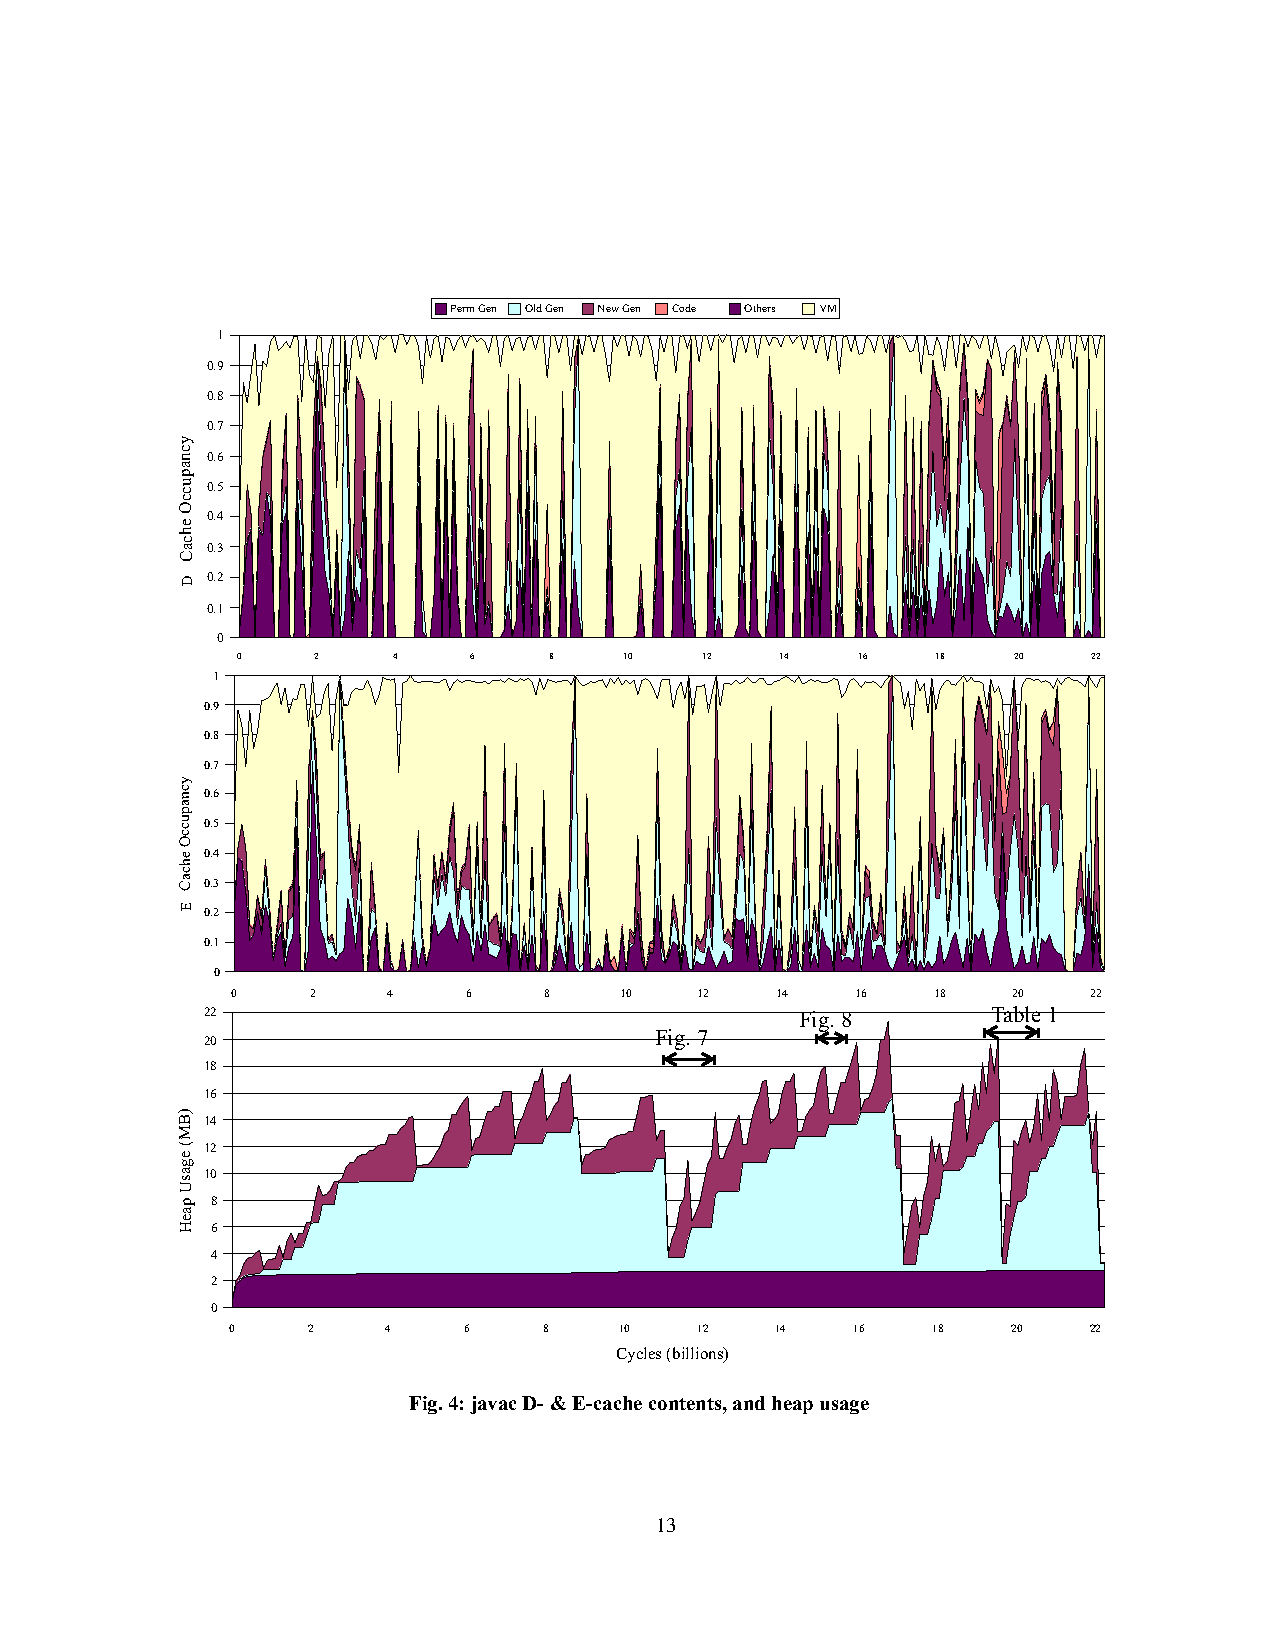
\includegraphics[width=\columnwidth, clip, trim=5cm 22.5cm 4.5cm 5cm]{heap}%
  \vspace{-1pt}
  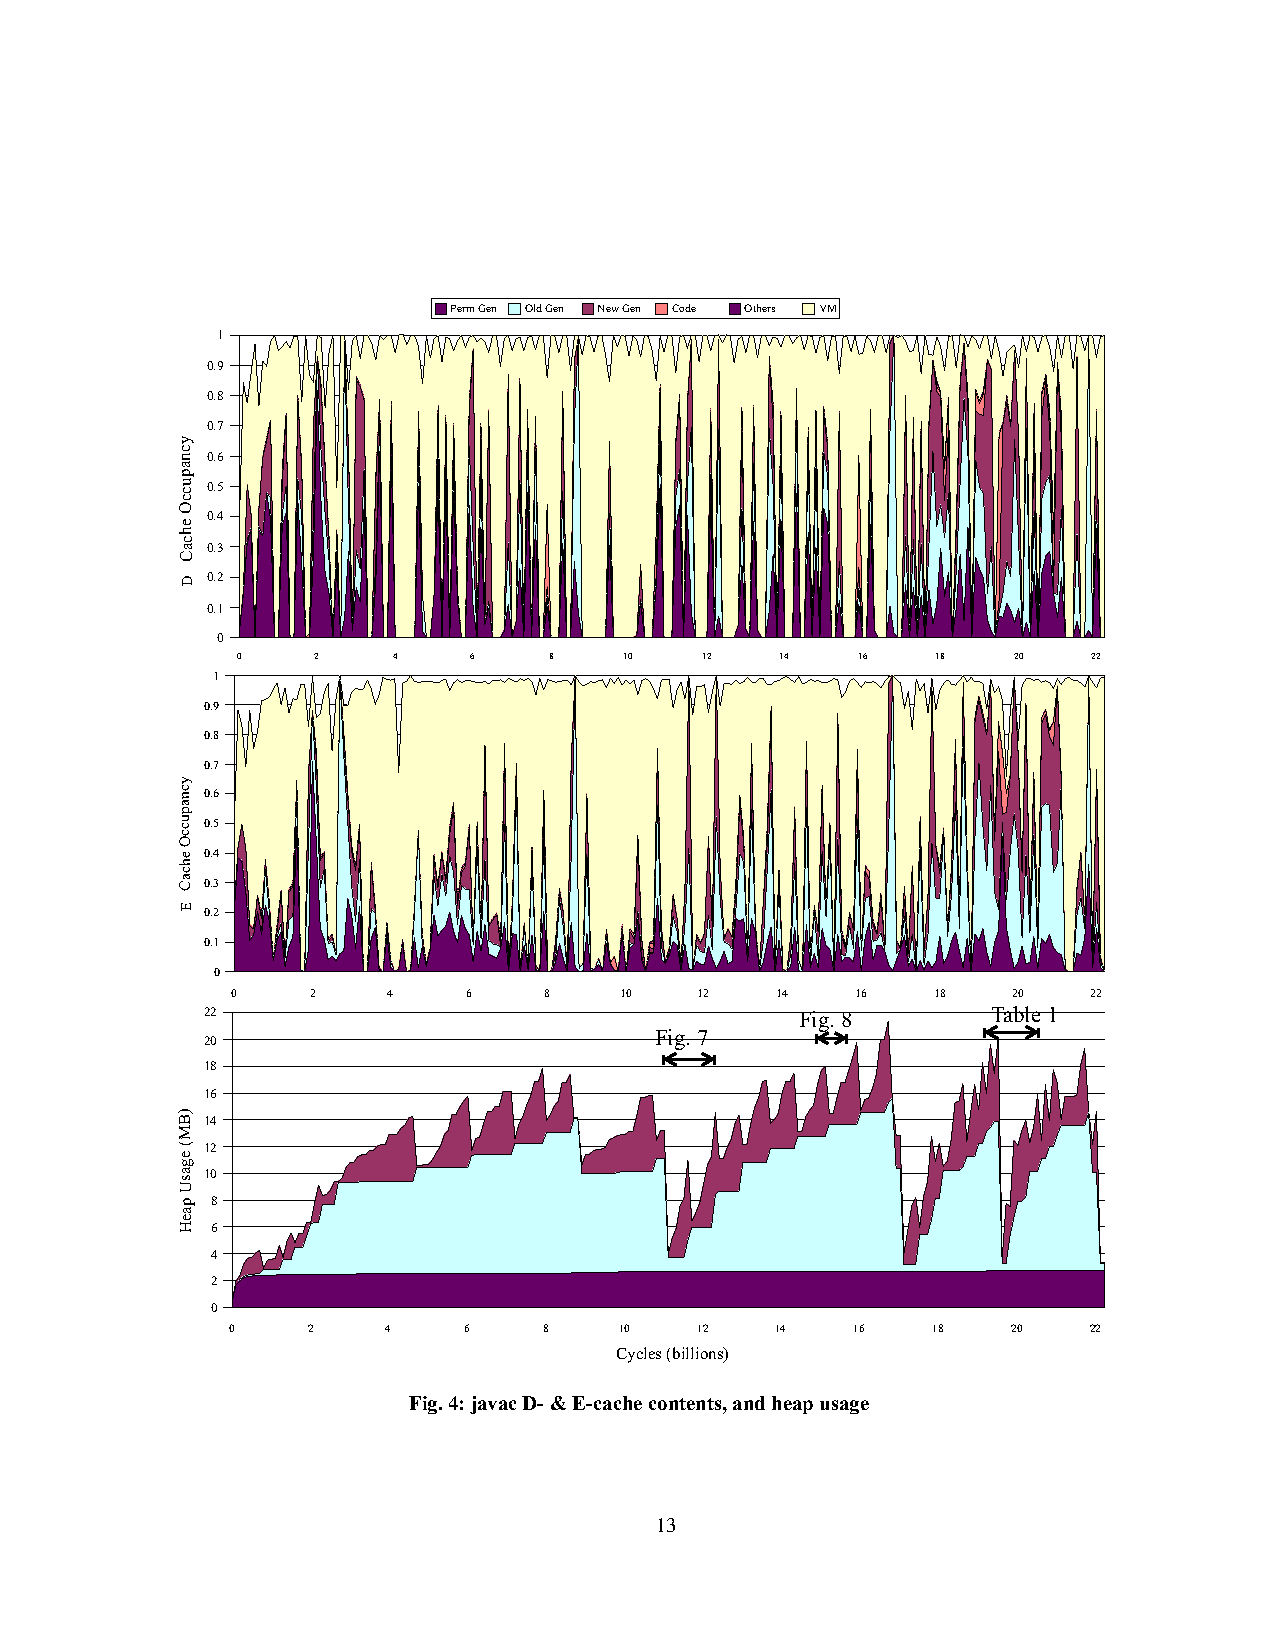
\includegraphics[width=\columnwidth, clip, trim=3cm 4.75cm 2.5cm 17cm]{heap}
  \src{Introspection of a Java Virtual Machine under Simulation, Wright et al, Sun Labs TR-2006-159}
\end{frame}

\begin{frame}{Tuning Generational Garbage Collectors}
  \begin{itemize}  \setlength{\itemsep}{\fill}
  \item Tenuring threshold
  \item Allocating directly to old space
  \item Size of generations
  \item Old space collectors
  \end{itemize}
\end{frame}

% Closing slide
% \subsection{Closure}
% % {
% % \setbeamertemplate{footline}{}
% % \begin{frame}[noframenumbering]
% %  \frametitle{\fontspec{Purisa}\textbf{Thank You!}}
% %  \centering
% %  \titlepage
% % \end{frame}
% % }
% \begin{frame}
%   % \centering
%   \Huge
%   \alert{Can managed programming languages run on future
%   many-core architectures?}
%   % \vspace{-2em}
%   \vfill
%   \begin{flushright}
%     \fontspec{Purisa}\structure{Thank You!}
%   \end{flushright}
% \end{frame}

%   BACKUP SLIDES

\end{document}
